\chapter{Et fremtidigt Aalborg}
Nedenstående afsnit vil behandle Aalborgs kommuneplan med primært fokus på Aalborgs Vækstakse, der er ét af fem hovedpunkter i kommuneplanen. En beskrivelse af de fire resterende fokuspunkter vil give en forståelse for, at kommunen har flere tanker om byens udvikling, og alle fem fokuspunkter har relevans for hinanden og gavner til byens udvikling.

\section{Kommuneplan}
En kommuneplan er kommunens overordnede plan for kommunens udvikling. Inden for en periode på 12 år fastlægger kommunen de overordnede mål og retningslinjer for kommunens udvikling såvel i byerne som i det åbne land \citep{kommuneplan1}. 
\newline
\newline
En kommuneplan består af; en hovedstruktur, retningslinjer, kommuneplanrammer, bilag og tilhørende planredegørelse. 
\newline \indent{     }  Hovedstrukturen er den overordnede, strategiske og sammenfattende fysiske plan for kommunen. Den fastlægger de overordnede mål for udviklingen inden for de enkelte sektorer for hele kommunen og for de enkelte områder \citep{kommuneplan1}.
\newline \indent{     }  Retningslinjerne udgør de overordnede rammer for kommuneplanlægningen. De fastsætter principperne for arealanvendelsen i kommunen, og danner ligeledes grundlag for kommunens administration af planlovens landzonebestemmelser, samt administrationen af kompetencer indenfor anden lovgivning, herunder natur-, miljø-, bygge- og vejlovgivningen og husdyrloven. Retningslinjerne angiver sammen med områdeudpegningerne hvilke forhold, der skal tages hensyn til i administrationen, og hvilke konkrete skøn der skal foretages for disse områder \citep{retningslinjer}. 
\newline \indent{     }  Kommuneplanrammerne styrer den overordnede arealanvendelse og danner ramme for indholdet i nye lokalplaner. Planrammerne fastlægger dermed mål, muligheder og begrænsninger for arealanvendelse i de enkelte dele af kommunen. Kommuneplanrammerne har to niveauer: 1) by/bydel/landområde og 2) rammeområder. Det første niveau “by/bydel/landområde”, behandler områdets særlige problemer, værdier og muligheder i en sammenhæng. Det andet niveau “rammeområder”, er det mest detaljerede niveau i kommuneplanen rent geografisk. Her fastsættes de bestemmelser, der danner grundlag for lokalplaner \citep{rammer}. 
\newline \indent{     }  Bilag er de generelle rammebestemmelser, hvor der henvises til de aktuelle bilag fra de enkelte emner \citep{bilag}.
\newline \indent{     }  Planredegørelser beskriver forudsætninger for, og ændringerne i den konkrete planlægning. Byrådet offentliggør, sammen med alle kommuneplanforslag eller med forslag til kommuneplantillæg\footnote{Opstår der problemer med at realisere en lokalplan ud fra kommuneplanen, så anvendes der et kommuneplantillæg, som er et supplement til den eksisterende kommuneplan. Denne kan justere og ændre bestemmelserne i kommuneplanen, for at gøre det muligt at realisere lokalplanen \citep{kommuneplan2009}.}, en redegørelse om planens baggrund og sammenhæng med anden planlægning. Kommuneplanen ledsages også af en planredegørelse og planstrategi, hvilken laves minimum hvert fjerde år i tilknytning til kommunens budget. Denne er byrådets instrument og baner vejen for at realisere kommuneplanens mål. Her oplyses blandt andet om kommuneplanens væsentlige forudsætninger, planlægninger der er gennemført det forgangne år, det kommende års kommuneplaninitiativer samt byrådets vurdering af og strategi for udviklingen for både det kommende år (budgetåret), de kommende fire år (overslagsårene) og en længere periode på 12 år. Desuden laves der jævnligt statusredegørelser, som giver et overordnet billede af kommunens fysiske udvikling og præsenterer de økonomiske tiltag, der knytter sig til kommunens sektorer og geografiske områder \citep{planredegorelse}.

\section{Aalborg Kommuneplan}
Aalborg Kommuneplan beskriver kommunens udvikling inden for de 12 kommende år og er opdelt i fem fokuspunkter: 
\begin{enumerate}
	\item Byerne - et godt sted at bo hele livet
	\item Nødvendige forbindelser - mobilitet
	\item Det åbne land
	\item Bæredygtighedsprofil
	\item Aalborg - den attraktive storby
\end{enumerate}
Et af Aalborg Kommuneplans fem fokuspunkter er "Byerne - et godt sted at bo hele livet". De større byer under Aalborg Kommune har, i kraft af nærheden til Aalborg, en god infrastruktur,  et varieret serviceudbud samt tilstrækkeligt befolkningsunderlag. Det er et særligt potentiale for byvækst, der skal udnyttes for at understøtte Aalborg som Norddanmarks Vækstdynamo. 
\newline \indent{     }  Byvæksten skal have særligt fokus på nye, kreative boligformer, som tilgodeser klimaudfordringer, demografiske udfordringer og bæredygtighed. 
\newline \indent{     }  Ikke kun de større byer nær Aalborg har en væsentlig rolle i projektet. Mindre byer og landsbyer er også i fokus, og har en særlig rolle som opland til Aalborg med store kvaliteter indenfor bosætning, rekreation og friluftsliv \citep{byerne}.
\newline
\newline
Et andet af Aalborg Kommuneplans fem fokuspunkter er “Nødvendige forbindelser - mobilitet”. Dette fokuspunkt omhandler byens behov for forbindelser, der kan håndtere transportbehovet og gøre det mere attraktivt at benytte offentlig transport såsom bus og tog, samt at tage cyklen, da  Aalborg Kommune har en målsætning om at blive Danmarks førende cykelby. Kommunens mål er færre bilkøer, god adgang til indkøb, service og arbejdspladser samt sikring af forbindelser, der understøtter en effektiv godstransport. Derudover satser Aalborg på en letbane som det bærende element i byen \citep{mobilitet}.
\newline
\newline
Fokuspunktet “Det åbne land” omhandler benyttelsen og beskyttelsen af det åbne land. Dette skal ske på et bæredygtigt grundlag med plads til oplevelser, natur, erhvervsinteresser og vedvarende energi. Det åbne land skal danne ramme om levende og aktive områder \citep{land}.
\newline
\newline
Aalborg Kommune har også stor fokus på bæredygtighed og har dertil punktet “Bæredygtighedsprofil”. Udviklingen af et bæredygtigt samfund omhandler flere punkter, såsom at passe på miljøet, klimaet og naturen, om at bygge byer for mennesker og om at få det bedste ud af den nuværende økonomiske virkelighed. En bred tilgang til bæredygtighed er derfor udgangspunktet \citep{profil}.

\subsection{Aalborg Vækstakse}
Det femte og sidste fokuspunkt i Aalborgs kommuneplan er “Aalborg - den attraktive storby”. Dette fokuspunkt indeholder yderligere tre punkter; vækstaksen som byens motor, byudviklingsprincipper for Aalborg og fokus på bykvalitet. 
\newline
\newline
Aalborg Kommune har valgt at koncentrere sig om et vækstbånd, kaldet Vækstaksen, som skal danne grundlag for Aalborgs udvikling, hvor der er fokus på det generelle udviklingsprincip \citep{kommuneplan3}. Området går fra Aalborg Lufthavn i vest, gennem midtbyen, til Campus og videre ud til østhavnen, hvilket illustreres på Figur \ref{fig:vaekstakse}. 
\newline \indent{     }  Blandt Vækstaksens mest centrale elementer er færdiggørelsen og videreudviklingen af en række større områder i Aalborg, som for fremtiden skal være med til at skabe Aalborg som storby og præge dens identitet. Gennem disse færdiggørelser vil bykvaliteten øges, og byen vil blive mere attraktiv. Der lægges derfor stor vægt på arkitektoniske overvejelser samt historiske skulpturer og monumenter, når der skal bygges og renoveres \citep{kommuneplan3}. 
\newline \indent{     }  Her har havnefronten, som et af de første områder, gennemgået en stor renovering, hvor der er etableret både Aalborg Havnebad, Jomfru Ane Parken og sportsfaciliteter. Derudover blev Tivoli Karolinelund fjernet i 2011, og i 2012 åbnede en ny Karolinelund park, som nu danner ramme for mange forskellige nichekulturer, såsom koncerter, Platform 4, legepladser og meget mere, og parken er fortsat under udvikling \citep{jomfruaneparken} \citep{karolinelund}. 
\newline \indent{     }  Aalborg er gennem renoveringen af den nye havnefront også vokset som kulturby, og i dag er kultur blevet en bærende del af byen, hvor der findes KUNSTEN Museum, Aalborg Kongres \& Kultur Center, Nordkraft samt det nye Musikkens Hus, der åbnede i 2014, hvor der hver uge afholdes forskellige koncerter og andre arrangementer. Dette er altsammen med til at styrke Aalborg som vækstby og byens erhvervsturisme \citep{kommuneplan3}. Ligeledes er der planer om en ny kulturbro på Jernbanebroen, som også skal være med til at styrke kulturen i Aalborg og Aalborg Kommune. Ved at styrke kulturen styrkes bykvaliteten også, og byen bliver en levende by, hvor det er muligt at binde shopping, café og kulturliv sammen \citep{kulturbro} \citep{musikkenshus}.
\newline \indent{     }  Den gamle Eternitgrund i Aalborg havde i en lang årrække stået ubrugt hen, men gennem de sidste fem år er der etableret både studieboliger, supermarkeder, fitnesscenter og et nyt legeland for børn. Virksomheder som Plus Bolig og COWI er ligeledes flyttet ned på Eternitten, og i dag er Eternitten blevet en stor drivkraft for Aalborg,  hvor der fortsat  er fremtidige planer om grønne arealer også \citep{eternitten}.
\newline \indent{     }  Projektet om Vækstaksen er i fuld gang, og inden for den nærmeste fremtid skal også Godsbanearealet og det østlige Aalborg udvikles, for at øge oplevelsesmulighederne, kulturtilbudene og skabe attraktive og bæredygtige livsvilkår her. Det er dog ikke kun nybyggerier, som Vækstaksen har fokus på. For Aalborg Kommune er det også vigtigt, at vedligeholde de gamle bygninger, for at opretholde byens historisk identitet \citep{kommuneplan3}.

\begin{figure}[htbp]
	\centering
	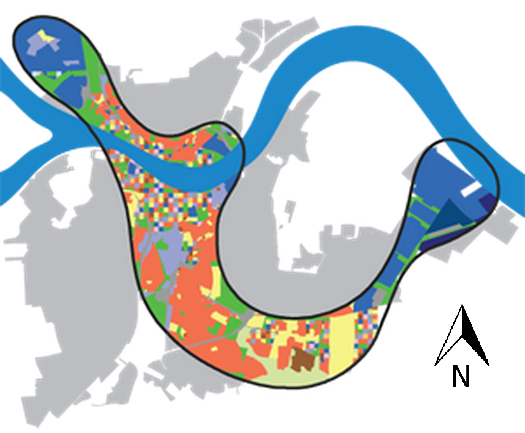
\includegraphics[width=0.5\textwidth]{billeder/vaekstaksen.png}
	\caption{Aalborgs Væsktakse \citep{kommuneplan3}}
	\label{fig:vaekstakse}
\end{figure}

Vækstaksen skal være attraktiv for alle aldersgrupper og skal derfor have noget at tilbyde hver enkelte borger, og skal ligeledes være med til at skabe oplevelsesmuligheder og kulturtilbud.
\newline \indent{     }  En stor del af planerne for Vækstaksen er byfortætning, mobilitet, studieby og miljø \citep{kommuneplan3}. 
Der er i Aalborg Kommune stor udviklingspotentiale inden for byfortætning. På Figur \ref{fig:udvikling} ses udviklingspotentialet i Vækstaksen. De markerede lilla områder er der hvor Aalborg Kommune har bedst udviklingspotentiale \citep{kommuneplan3}.
\newline \indent{     }  Dette udviklingspotentiale er i form af tilbyggelse og omdannelse af boliger, arbejdspladser og naturområder. Byfortætning kan resultere i en meget presset infrastruktur, derfor er mobilitet et essentielt punkt for optimering af byens potentiale \citep{kommuneplan3}. Det er vigtigt, at der er let og hurtigt adgang til offentlig transport, og det skal gøres mere attraktivt, at tage cyklen. Målet er, at få en stor by til at opfattes som en “lille by”, ved at gøre transport lettilgængeligt og derfor nemt at komme fra bydel til bydel. Infrastrukturen vil styrkes blandt andet via en cykelmotorvej samt en kommende letbane, som skal forbinde Østhavnen, Campus, det kommende superhospital i Aalborg Øst, midtbyen og ud til Aalborg Lufthavn \citep{kommuneplan3}.

\begin{figure}[htbp]
	\centering
	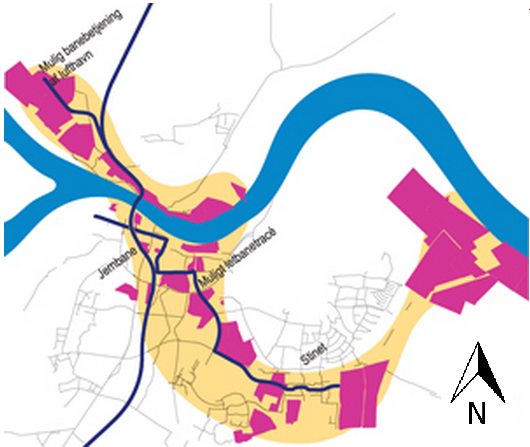
\includegraphics[width=0.5\textwidth]{billeder/udvikling.png}
	\caption{Udviklingspotentiale \citep{kommuneplan3}}
	\label{fig:udvikling}
\end{figure}

Ved Vækstaksens to endepunkter ligger Aalborgs største industriområder, Aalborg Østhavn og Aalborg Lufthavn. Disse industriområder er kommet til, efter industrifirmaer er begyndt at flytte fra havnefronten og ud til yderkanten af Vækstaksen. Trods denne flytning forbliver Aalborg en erhvervsby samtidig med, at den gradvist omdannes til en studieby. De store industrifirmaer er stadig vigtige for Aalborg, da de er med til at skabe omsætning og arbejdspladser \citep{kommuneplan3}. 
\newline \indent{     }  Da Aalborg gradvist omdannes til en studieby, er det vigtigt, at der i Vækstaksen støttes op om Aalborgs studieliv og studiemiljø, da 10\% af Aalborg Kommunes befolkning består af studerende \citep{campus}. Et godt studiemiljø vil styrke innovation, konkurrence og vækst i erhvervslivet. Det er nødvendigt med gode uddannelsesmuligheder, faciliteter samt ungdomsboliger til de studerende, hvilket også vil gøre det attraktivt for udefrakommende at studere i Aalborg. Centrum for studielivet i Aalborg udspringer fra Campus i Aalborg Øst, hvor størstedelen af de videregående uddannelser findes \citep{kommuneplan3}. 
\newline
\newline
Aalborg Kommune ønsker også at udvikle byens natur og udendørsliv. Til at opnå dette vil kommunen opføre parker, stisystemer og vandløb. Vandløbene vil give byen historisk identitet, samtidig med at de vil beskytte byen under eventuel øget vandstand, da de kan forsinke vandet \citep{kommuneplan3}. Formålet med parkerne og et naturrigt Aalborg er at skabe et sundhedsfremmende forhold for alle aldersgrupper og beskytte klimaet. Desuden vil Aalborg Kommune gøre Aalborg til en miljøvenlig storby, som antages at gøre byen mere attraktiv, og dermed øge indbyggertallet. Derfor vil Aalborg Kommune genoprette naturen og give velfærd til byens borgere \citep{kommuneplan3}.

\section{Vækstaksens betydning}
Formålet med Vækstaksen er, at styrke Aalborg som by, og der er en forventning fra Aalborg Kommune om, at byen bliver Nordjyllands Vækstdynamo, men er dette realistisk? Nedenstående afsnit vil stille spørgsmålstegn ved Vækstaksen, og diskutere, hvilken sammenhæng Strøybergs Palæ og Vækstaksen har med hinanden. I den forbindelse vil der diskuteres, hvorfor der ønskes en tilbygning, og hvorfor det netop er i dette område, det er fordelagtigt at udvide.

\subsection{Er visionerne realistiske?}
Vækstaksen er placeret således, at den går gennem Aalborgs centrale områder for kultur, uddannelse, erhverv og miljø.  Aalborg Kommune ønsker at etablere en god infrastruktur, som den kommende Letbane for eksempel skal hjælpe med \citep{kommuneplan3}. Det er fordelagtigt at udvide samt udvikle i Vækstaksen, da områderne samt virksomhederne er drivkraften for Aalborg \citep{bedreoverblik}, og det er her, at byens liv er, og fremtiden skal skabes. Selvom områderne i dag fungerer som drivkraft, skal disse stadig videreudvikles, da Aalborg er en by i stor vækst, hvilket afspejles af både stigende indbyggertal og antal virksomheder, som flytter til og skabes i Aalborg \citep{statistik}\citep{virksomheder}. Derfor kan Aalborg Kommune ikke blot stille sig tilfreds med de nuværende tilstande, da byen skal udvides, for at være forberedt på fremtiden; ellers er der ikke plads til udviklingen, og den vil bremses, gå helt i stå eller i værste fald gå den anden vej.
\newline \indent{     }  Udviklingen af byen vil primært ske gennem en byfortætning, da de centrale områder allerede i dag er fyldt med liv samt kultur, erhverv og uddannelse. Der er altså ikke tale om store udvidelser af områderne, men snarere optimeringer af de allerede eksisterende områder, og derfor kan infrastrukturen opleve problemer. 
\newline \indent{     }  I takt med at indbyggertallet stiger kan det formodes at antallet af biler vil stige. Derfor kan spørgsmålet stilles, om det er realistisk med en fortætning af byen samtidig med, at Aalborg Kommune har en målsætning om, at det skal være let at færdes i byen som fodgænger, cyklist og med offentlig transport \citep{kommuneplan3}. Dette afspejler sig i trafikken omkring Nyhavnsgade, som strækker sig fra Nordkraft forbi Strøybergs Palæ og videre langs med havnefronten. Her er vejen ændret fra en 4-sporet vej til en 2-sporet. Derfor er antallet af bilister næsten halveret, fra 20.500 (ÅDT) til 11.000 (ÅDT), og hastigheden er sænket \citep[ s. 6]{lokalplan}. Selvom Aalborg Kommune har sænket antallet af bilister omkring centrum, så vil en udvikling af byen og et øget indbyggertal betyde, at flere bilister igen vil køre gennem centrum, så trafikken igen vil begynde at stige. Derfor har Aalborg Kommune kun løst problemet delvist, for med tanke på en kommende vækst for byen så øges årsdøgntrafikken. Det betyder, at Aalborg Kommune igen vil stå med et problem, hvis ønsket om at opretholde et lavt antal bilister samt at det skal være let at færdes i byen for de bløde trafikanter, skal imødekommes. Nu er det blot ikke muligt at skære ned på antallet af kørespor, og derved skal der findes en ny løsning, med mindre Aalborg Kommune ændrer synspunkt på problemet.
\newline \indent{     }  Aalborg Kommune ønsker færre biler omkring centrum, for at gøre det mere attraktivt og lettere for de bløde trafikanter at færdes \citep{aalborgletbane} \citep{nordjyske}. Letbanen vil gøre det mere attraktivt at undvære bil i Aalborg, men i takt med fortætningen er spørgsmålet, om det er nok, til at det føles let at færdes i Aalborg. Et andet fokuspunkt er en tredje Limfjordsforbindelse, som der i dag er ønske om \citep{limfjordsforbindelsen}. Trafikken i morgen- og eftermiddagstimerne til og fra Aalborg er tæt, og særligt når der opstår et trafikuheld i en af Limfjordsforbindelserne for køretøjer over Limfjorden, så opstår der trafikale problemer omkring den anden forbindelse, og centrum bliver overbelastet. Dette kan en tredje Limfjordsforbindelse afhjælpe, da den af naturlige årsager vil medføre flere biler på vejen, og omvendt vil trafikken også blive mere jævn fordelt, da der kommer en ekstra strækning, som bilisterne kan anvende. Dette kan gavne Aalborg Centrum, både ved den daglige trafik omkring centrum, og ved et eventuelt uheld i Limfjordstunnelen, da det ikke længere kun vil være centrum, der så giver adgang for bilister til at passere over på den anden side af fjorden. Her vil en tredje forbindelse så også vil kunne anvendes, og dermed lette trafikken. 
\newline
\newline
Aalborg har et ønske om at være Danmarks bedste studieby \citep{ungdom}, og derfor kræves der nok studieboliger til de studerende. Der er i landet en generel mangel på studieboliger, og dette gør sig også gældende for Aalborg, selvom det ikke er i ligeså høj grad som eksempelvis København. Det skyldes Aalborgs store fokus på de studerende og behovet for studieboliger, hvoraf der er blevet bygget over 6.000 studieboliger siden 2010 inden for Vækstaksen, både på Aalborg og Nørresundby siden, og der bygges fortsat flere nye boliger i dag \citep{studieboliger}. Dette er et led i Vækstaksen og planerne om Aalborgs fremtid. De seneste fem år har de videregående uddannelser oplevet rekordmange ansøgninger og dermed flere studerende \citep{uddannelser}, hvilket betyder, at studieboligerne hurtigt bliver lejet ud. Der er fra år 2009 til 2014 kommet ca. 8.000 flere studerende til \citep[ s. 9]{unital}. Et af kommunens fokuspunkterne er, at gøre Aalborg en attraktiv studieby med studievenlige priser på boligerne. Sammenlignes priserne med de tre andre storbyer i Danmark; Aarhus, Odense og København, er boligerne i Aalborg væsentlig billigere \citep{home}, hvilket kan være en medvirkende faktor til, at Aalborg er attraktiv for de unge.
\newline
\newline
Aalborg Kommune har også et ønske om, at byen skal være for alle mennesker i alle aldersgrupper samt et attraktivt sted for erhverv \citep{kl} \citep{kommuneplan3}. Spørgsmålet er dog, hvor erhverv skal etableres inden for Vækstaksen, og hvad der kan gøres for de indbyggere, som ikke er studerende. Havnefronten, som er en af de bærende elementer i Vækstaksen, anvendes ikke kun af unge, men også af børnefamilier. Derudover byder Aalborg også på naturområder og attraktioner, som er for alle i alle aldersgrupper.
\newline
\newline
For nye virksomheder gælder det, at der skal være kontorlokaler og bygninger, som kan huse virksomhederne. Ligeledes skal virksomhedens beskæftigelse gerne passe med Aalborg, således at der er en sammenhæng mellem kunde og virksomhed. Med en målsætning om, at være en attraktiv storby med mange muligheder for virksomheder, er der derfor et godt grundlag for at drive virksomhed i Aalborg, også i fremtiden. Indenfor Vækstaksen ligger der utallige virksomheder, men der er stadig tomme erhvervslokaler, som vil give plads til flere virksomheder. Heriblandt skal der ske en udvidelse af Strøybergs Palæ, som har en central beliggenhed i Vækstaksen, helt nede ved havnefronten.

\subsection{Hvorfor udvide Strøybergs Palæ?}
Strøybergs Palæ ligger i Vækstaksen. På Figur \ref{fig:udvikling} ses det, at Strøybergs Palæ ligger i det lilla område og er dermed i et område, hvor der er størst mulighed for udvikling inden for Vækstaksen. Grundet havnefrontens udvikling de sidste 10 år, har der været fokus på udviklingen her, og nu har Aalborg Kommune godkendt forespørgslen om en tilbygning til Strøybergs Palæ, da der allerede er bygget Musikkens Hus, havnefronten, Utzon Centeret og Utzon Parken omkring området. Udviklingen omkring havnefronten er sket i takt med Vækstaksens fokus herpå. Om havnefronten havde fået en udvikling overhovedet eller i lige så høj grad, hvis tankerne og ideérne omkring Vækstaksen ikke var blevet sat i værk, kan diskuteres. Uden en vækstakse vil der stadig ske en udvikling ved havnefronten, men ikke i ligeså høj grad, som nu, hvor Vækstaksen bringer ekstra fokus på området. Dog må det formodes, at havnefronten ikke vil udvikle sig i samme retning i forhold til de kulturmæssige fokuspunkter som Vækstaksen giver. 
\newline \indent{     }  Det kan ligeledes diskuteres om Vækstaksen overhovedet har haft indflydelse på udvidelsen af Strøybergs Palæ. Placeringen af Strøybergs Palæ midt i Vækstaksen, kan tænkes at have haft indflydelse på beslutningen om, at der skal laves en tilbygning, fordi bygningen skal leve op til Aalborg Kommunes forventninger, og ønsker for fremtiden. Tilbygningen kan bruges til erhvervslokaler, og dette vil kunne tiltrække en eller flere nye virksomheder til området, og dermed være med til at udvikle både området og Aalborg by. Omvendt kan spørgsmålet dog også stilles, om denne tilbygning vil få den ønskede effekt og kunne leve op til disse målsætninger. Det vil være naivt at tro, at en udvidelse på nogle få hundrede kvadratmeter vil gøre en betydende forskel for Aalborg, og det kan derfor ikke alene være grunden til tilbygningen, men snarere en af flere årsager. Strøybergs Palæ er kun en lille del af Vækstaksen, og skal derfor ikke bære Aalborgs udvikling og vækst alene.
\newline \indent{     }  Hovedpunkterne i Vækstaksen er, at Aalborg skal vokse som by, og udvikles gennem en byfortætning, hvor målet er, at tiltrække flere  virksomheder og indbyggere. En udvidelse af Strøybergs Palæ vil give ekstra erhvervslokaler og/eller lejligheder, og dette passer godt sammen med Vækstaksen. Tilbygningen betyder desuden, at Strøybergs Palæ vil få et mere harmonisk udseende ud mod vandet, da tilbygningen vil blive bygget i samme arkitektoniske stil som resten af bygningen, og den nordøstlige del af bygningen vil komme op i cirka samme højde, som resten af bygningen. Sammen med resten af havnefronten vil Strøybergs Palæ gennemgå en renovering, som løfter udseendet samt medfører, at området vil få en mere ensformet og harmonisk stil.
\newline \indent{     }  Det, at området bliver et centralt fokuspunkt for fremtiden betyder også, at området bliver mere attraktivt, idét der kommer til at ske en fortsat udvikling af området, og netop derfor kan en tilbygning være en god investering, da det giver ekstra plads og bedre forudsætninger for udviklingen.